% 1977 年江苏镇江地区初试卷第 6 题：测量不能直接到达底部的高塔 AB，
% 地面基线 CD、望塔顶 A 与塔基 B 的视线示意图（按源卷第 2 页布局）
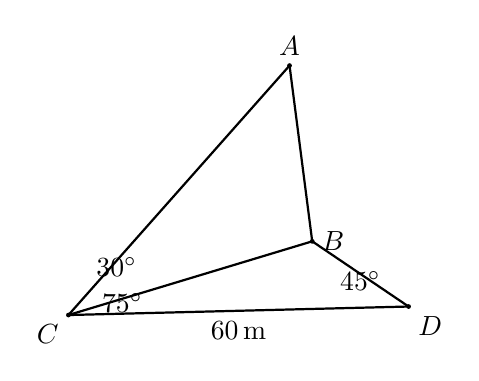
\begin{tikzpicture}[scale=0.72,>=stealth]
  \coordinate (C) at (0,0);
  \coordinate (D) at (6,0.15);
  \coordinate (B) at (4.3,1.3);
  \coordinate (A) at (3.9,4.4);
  \draw[thick] (C)--(A);
  \draw[thick] (C)--(B);
  \draw[thick] (C)--(D);
  \draw[thick] (D)--(B);
  \draw[thick] (A)--(B);
  \fill (A) circle (1.2pt) node[above] {$A$};
  \fill (B) circle (1.2pt) node[right] {$B$};
  \fill (C) circle (1.2pt) node[below left] {$C$};
  \fill (D) circle (1.2pt) node[below right] {$D$};
  \node at (0.85,0.85) {$30^\circ$};
  \node at (0.95,0.22) {$75^\circ$};
  \node at (5.15,0.6) {$45^\circ$};
  \node[below] at (3,0.05) {$60\,\mathrm{m}$};
\end{tikzpicture}
